\documentclass{article}
\title{Blanchard Ch.4}
\author{Dawei Wang}
\date{\today}
\usepackage{ctex}
\usepackage{amsmath}
\usepackage{amssymb}
\usepackage{graphicx} %插入图片的宏包
\usepackage{float} %设置图片浮动位置的宏包
\usepackage{subfigure} %插入多图时用子图显示的宏包
\begin{document}
	\maketitle
\section{货币需求}
假设人们在现金和债券中选择投资组合。(假设债券交易有交易成本)
\hspace*{\fill}

货币,可以用来交易,但不支付利息。现实生活中包括两种货币:通货(currency)和可开支票的存款(checkable deposits)。

债券,要支付利息,但不能用于交易。设其利率为i。

\hspace*{\fill}

在货币和债券之间的持有比例的决定因素:

1. 交易水平(取决于经济状况,交易水平高,货币需求高);

2. 债券利率(利率高,货币需求低)。

\hspace*{\fill}

大多数人并不直接持有债券,许多人都是通过货币市场基金间接持有债券。

\hspace*{\fill}

语义分析:

货币:能够用于交易支付,包括通货和可开支票的活期存款;

收入:流量,工作报酬加上获得的利息和红利;

储蓄:流量,税后收入中没有被花费的那一部分(也可指存量,为财富同义词);

金融财富:存量,是指所有金融资产减去金融负债的价值;

可以直接用来购买商品的金融资产被称为货币(存量);

投资:在经济学中用来表示购买新资本品(机器、厂房);购买金融资产时叫作金融投资。

\subsection{货币需求的推导}
用$ M^d $表示人们想要持有的货币数量,即货币需求。经济中货币需求整体上等于所有个人的货币需求之和,因此,整个经济的货币需求取决于经济中的整体交易水平和利率。经济中的整体交易水平与名义收入大致成比例关系(影响货币需求的是名义收入,以美元表示的收入,而不是实际收入)。因此,货币需求、名义收入和利率的关系为:
\[
M^d=\$YL(i)
\]
其中$ \$Y $表示名义收入$ L(i) $为利率的函数。

既定名义收入的情况下,货币需求与利率之间的关系由$ M^d $曲线表示,曲线向下倾斜:利率越低,人们想要持有的货币越多。

货币需求的增加同名义收入的增加成正比例。如果名义收入增加一倍,从\$Y增加到\$2Y,那么货币需求也增加一倍,从\$YL(i)增加到2\$YL(i)。

对于给定利率,名义收入的增加将提高货币需求——名义收入的增加将导致货币需求曲线右移。

\section{利率的决定:\uppercase\expandafter{\romannumeral1}}
现实中有两个货币供给者:银行提供可开支票的存款,中央银行提供通货。现不考虑可开支票的存款。

\subsection{货币需求、货币供给和均衡利率}

假设中央银行决定的货币供给量为M,因此
\[
M^s=M
\]

金融市场均衡条件:$ M^s=M^d $即:
\[
M=\$YL(i)
\]

该等式意味着利率必须使人们愿意持有的货币数量等于已有的货币供给。这一均衡关系被称为LM关系。其中L代表流动性(liquidity),M代表货币。

货币供给曲线$ M^s $与货币需求曲线$ M^d $的交点的利率就是均衡利率。

给定货币供给量,名义收入的上升(提高交易水平)将导致利率的上升。

给定名义收入,货币供给量的增加将导致利率的下降。

\subsection{货币政策与公开市场操作}
公开市场操作:

中央银行通过购买或者出售债券来改变经济中的货币数量。如果想要增加经济中的货币数量,可以通过发行货币来购买债券;如果想要减少经济中的货币数量,就出售债券,用债券换回流通中的货币。这种行为被称为公开市场操作(open market operations),这些业务均发生在债券的“公开市场”中。

中央银行的资产为其资产组合中的债券,负债为经济中的货币存量。中央银行购买债券(增加货币供给)的业务被称为扩张性公开市场操作(expansionary open market operations);中央银行出售债券(减少货币供给)的业务被称为紧缩性公开市场操作(contractionary open market operations)。

\hspace*{\fill}

法定准备金率=reserve/deposit

\hspace*{\fill}

再贴现率:商业银行用未到期票据向央行申请贴现的预扣利率

\subsection{债券价格和债券收益}
扩张性公开市场操作:央行购买债券(货币供给增加)$ \rightarrow $债券价格上升$ \rightarrow $利率下降;

紧缩性公开市场操作:央行出售债券(货币供给减少)$ \rightarrow $债券价格下降$ \rightarrow $利率上升。

\subsection{选择货币还是选择利率}
先前的描述是:中央银行先选择货币供给量,然后再货币供给等于需求的那一点确定利率。相反,也可以理解为:中央银行首先选择利率,然后再调整货币供给以实现这一利率。

注:短期利率(受央行控制)不是影响支出的唯一利率。

\subsection{货币、债券和其他资产}
短期利率由货币供给等于货币需求这一条件决定;中央银行可以通过公开市场操作来改变货币数量和短期利率;公开市场操作是绝大多数中央银行用来影响利率的基本工具。

\section{利率的决定:\uppercase\expandafter{\romannumeral2}}

\subsection{银行做些什么}
金融中介(financial intermediaries)从人们或企业手中筹集现金,并用这些资金购买债券或股票或者向其他人或企业发放贷款。它们的负债是向人们或者企业收取的资金,它们的资产是自己所有的金融资产以及发放的贷款。

银行为金融机构的一种,它的负债为货币:人们根据他们账户中的余额开出支票。

\hspace*{\fill}

银行持有准备金的原因:

1. 满足存款者的存取现金的需求;

2. 满足存款者银行间转账的需求;

3. 法律规定银行必须保留一定比例(法定准备金率)准备金。

\subsection{中央银行货币的供给与需求}
中央银行的货币需求=人们的通货需求+银行的准备金需求;

中央银行货币的供给处于中央银行控制之下;

均衡利率就是中央银行的货币供给等于需求时的利率。

\hspace*{\fill}

1. 货币需求
\[
M^d=\$YL(i)
\]
假设人们持有固定比例c的通货,1-c的可开支票存款:
\[
CU^d=cM^d
\]
\[
D^d=(1-c)M^d
\]
可开支票存款需求导致了银行的准备金需求。

\hspace*{\fill}

2. 准备金需求

可开支票存款的数量越大,银行必须持有的准备金越多。用$ \theta $表示准备金比率、R表示银行的准备金数量,D表示可开支票存款的数量。
\[
R=\theta D
\]
因此银行准备金需求为:
\[
R^d=\theta(1-c)M^d
\]

\hspace*{\fill}

3. 中央银行面临的货币需求
\[
H^d=CU^d+R^d
\]
\[
H^d=cM^d+\theta(1-c)M^d=[c+\theta(1-c)]M^d
\]
\[
H^d=[c+\theta(1-c)]\$YL(i)
\]

\hspace*{\fill}

4. 利率的决定

H代表中央银行的货币供给,中央银行直接控制H,均衡时有:
\[
H=H^d
\]
\[
H=[c+\theta(1-c)]\$YL(i)
\]

上式即决定了均衡利率。

当$ 0<c<1 $,中央银行的货币需求小于总的货币需求。因为事实上银行的准备金需求仅为可开支票存款需求的一部分。

\begin{figure}[H] %H为当前位置,!htb为忽略美学标准,htbp为浮动图形
	\centering %图片居中
	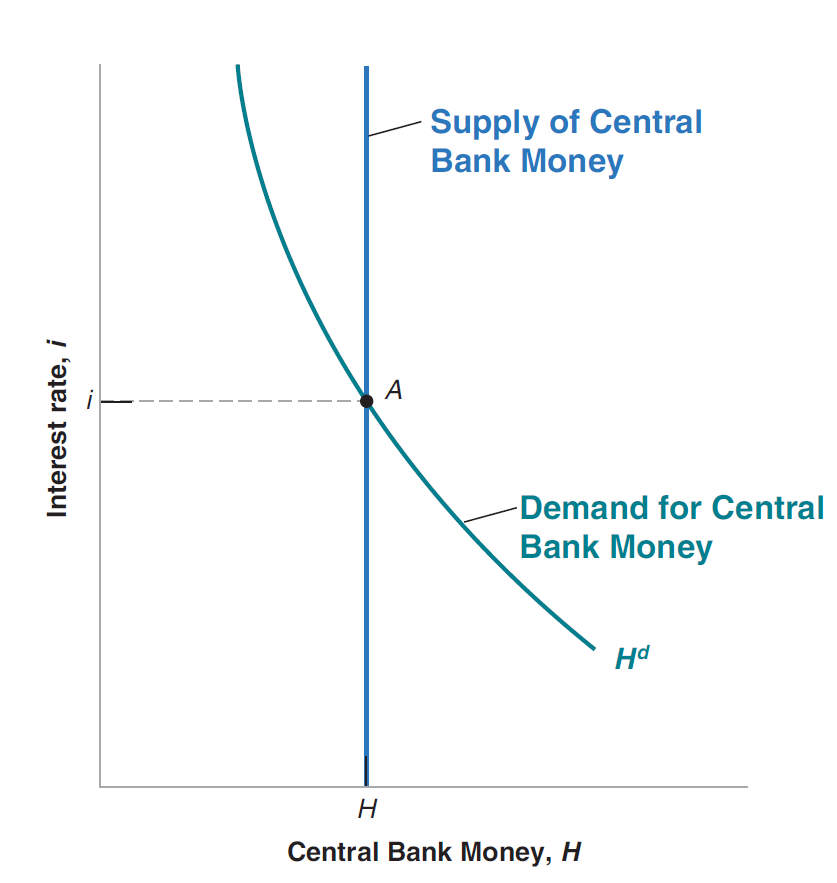
\includegraphics[width=1\textwidth]{4_2} %插入图片,[]中设置图片大小,{}中是图片文件名
	\caption{Equilibrium in the Market
		for Central Bank Money
		and the Determination of
		the Interest Rate} %最终文档中希望显示的图片标题
	\label{Fig.main3} %用于文内引用的标签
\end{figure}

\section{讨论均衡的两种方法}
\subsection{联邦基金市场和联邦基金利率}
考虑银行准备金的需求和供给:
\[
H-CU^d=R^d
\]

美国的准备金市场即为:联邦基金市场,该市场上利率不断调整以使准备金供给等于准备金需求,该市场被称为联邦基金市场。联邦基金市场的利率为联邦基金利率,联储可以通过改变中央银行货币供给来选择联邦基金利率。

\subsection{货币供给、货币需求和货币乘数}
将式:
\[
H=[c+\theta(1-c)]\$YL(i)
\]
变形:
\[
\frac{1}{[c+\theta(1-c)]}H=\$YL(i)
\]
上式左边为货币供给,右边为货币需求。

其中$ \frac{1}{[c+\theta(1-c)]} $被称为货币乘数(通常大于1),$ H $被称为高能货币或基础货币。

\hspace*{\fill}

$ M_0 $:现金(流通中的现金)

$ M_1 $:现金+活期存款(狭义货币供应量)

$ M_2 $:(广义货币供应量`)

\section{流动性陷阱}

利率不能处在零以下的水平,即零利率下限(zero lower bound)的约束条件:当利率趋于零时,货币政策不能进一步降低利率。这时货币利率失灵,经济中将这一现象称为流动性陷阱(liquidity trap)。

在利率为零时,人们如果为了交易的目的的需要持有货币,这时以货币形式持有的其他金融财富与持有债券形式的金融资产是没有差异的。没有差异的原因就是利率为零,货币和债券得到的支付是一样的,即都是零。

\begin{figure}[H] %H为当前位置,!htb为忽略美学标准,htbp为浮动图形
	\centering %图片居中
	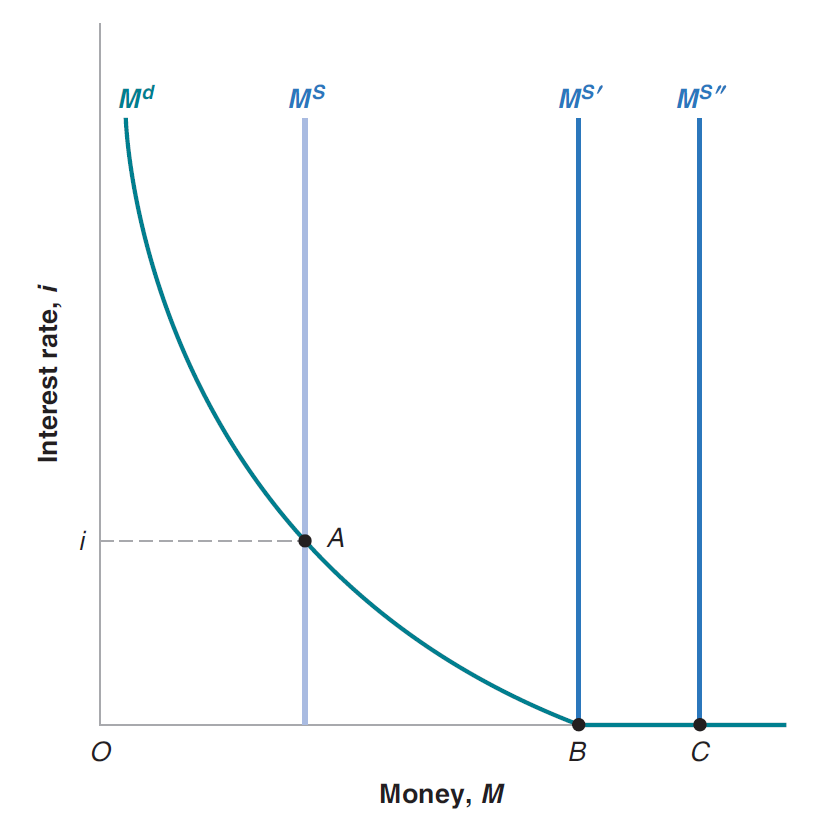
\includegraphics[width=1\textwidth]{4_1} %插入图片,[]中设置图片大小,{}中是图片文件名
	\caption{Money Demand, Money
		Supply, and the Liquidity
		Trap} %最终文档中希望显示的图片标题
	\label{Fig.main2} %用于文内引用的标签
\end{figure}

当利率下降时,人们愿意持有更多的货币(较少的债券),货币需求就会增加。

当利率需求为零时,人们想持有一定量的货币,至少是等于图中的距离OB。但是他们也愿意持有更多的货币。这是由于货币与债券在这时是没有差异的。因此货币需求在B点外是水平的。

考虑银行,银行的决策是持有准备金还是购买债券。如果利率为零,银行持有准备金与持有债券是没有差异的,两者得到的利息都是零。因此,当利率下降至零时,中央银行增加货币供给时,我们很有可能看到的是短期存款增加或者是银行准备金增加,利率仍然维持为零。








\end{document}